\documentclass{article}

\usepackage[final]{neurips_2018}

\usepackage{float}
\usepackage[utf8]{inputenc} % allow utf-8 input
\usepackage[T1]{fontenc}    % use 8-bit T1 fonts
\usepackage{hyperref}       % hyperlinks
\usepackage{url}            % simple URL typesetting
\usepackage{booktabs}       % professional-quality tables
\usepackage{amsfonts}       % blackboard math symbols
\usepackage{amsmath}
\usepackage{nicefrac}       % compact symbols for 1/2, etc.
\usepackage{microtype}      % microtypography
\usepackage{dsfont}
\usepackage{graphicx}
\graphicspath{ {./figs/} }

\usepackage[backend=biber, style=authoryear, citestyle=authoryear]{biblatex}
\addbibresource{main.bib}

\title{Magnitude autoencoder}

\author{%
  Tadas Bareikis\\
  ETH Zurich, D-BSSE\\
  \texttt{tbareikis@student.ethz.ch} \\
}

\begin{document}

\maketitle

\begin{abstract}
  This report presents the results of a 6-week-long lab rotation, the goal of which was to construct an autoencoder neural network with a focus on a data property called the weighting vector, which can be used as a boundary detector of a dataset. The autoencoder is used to reduce the dimensionality of a high-dimensional input dataset while using the weighting vectors of both representations in order to preserve the same boundary in both high and low dimensional datasets. Some basic and easily interpretable datasets are investigated to see how such an autoencoder performs in different scenarios. After seeing that these examples show that the autoencoder works in principle, it is then applied to the MNIST dataset, a real-world example.
\end{abstract}

\section{Introduction}

A finite metric space is defined as a pair of a finite set $X$ and a metric $d$ defining the distance between any pair of points from $X$. Such a space can be characterized by magnitude (\cite{Leinster2010}), a real-valued scalar quantity describing the effective number of points in the space. An intermediate object in the calculation of magnitude is the weighting vector, which assigns a value to each point in the space. The weighting vector has a useful feature for data analysis - it characterizes the structure of the original metric space by highlighting its boundary (\cite{Bunch2021}). For a dataset representing a shape, which is manifested as a point cloud, the weighting vector assigns low values for points interior to the shape and high values to points which lie on the boundary of the shape. Acting as a boundary detector, the weighting vector can be used to find outliers in the data.

A novel application of the weighting vector presented in this report is in dimensionality reduction. The boundary is a defining property of the structure of a dataset, therefore, it would be desirable to preserve it when visualizing a two-dimensional representation of the original high-dimensional dataset. The method chosen to perform dimensionality reduction is the autoencoder neural network. In order to ensure that the boundary present in the high-dimensional dataset is preserved in the two-dimensional representation, an additional loss term is introduced, which accounts for the differences between the weighting vectors of the two, high-dimensional and two-dimensional, representations.

The training of the neural network, however, is complicated by the fact that the boundary of a shape is a global property, and the calculation of the weighting vector is only meaningful when taking all of the dataset into account. This puts a restriction on how efficiently the neural network is trained, since each training epoch has to make use only of the whole dataset included into a single batch. Additionally, the calculation of the weighting vector for a dataset composed of $n$ points involves the inversion of a $n$ by $n$ similarity matrix, an operation with time complexity of $O(n^3)$, which becomes prohibitively expensive  for datasets containing many data points.

In this report, we demonstrate how a simple autoencoder training scheme works in principle on different datasets with a limited number of data points, and we also investigate how this procedure can be improved to address the stated problems which cause the training of the autoencoder to be inefficient.

\section{Theory}

\subsection{Magnitude}

A metric space consists of a set $X$ and a metric $d$. If $X$ has a finite number of elements, then the metric space is also finite, and we can calculate a similarity matrix $\zeta_{X} \in \mathbb{R}^{NxN}$ (\cite{Bunch2021}), where the similarity between points $a$ and $b$ in $X$ is defined as $$\zeta_{X}(a, b) = \exp{(-d(a, b))}.$$ Then, using such a similarity matrix we can calculate the weighting vector and magnitude of $X$ using the inverse of $\zeta_{X}$ : $$w_{X} = \zeta_{X}^{-1} \mathds{1} \text{ and } \text{Mag}(X) = \mathds{1}^{T} w_{X} ,$$ where $\mathds{1} \in \mathbb{R}^{Nx1}$ is a column vector of ones. Magnitude is a scalar value, which can be interpreted as the effective number of points \cite{Leinster2010}. For example, $X$ containing two points has magnitude equal to $\text{Mag}(X) = 1 + \tanh(d/2)$, where $d$ is the distance between the two points. If $d$ is very small, the magnitude of $X$ is close to 1, $X$ effectively represents a single point, since the two points contained in $X$ are very similar. On the other hand, if the points are dissimilar enough, $d$ is large, and the magnitude of $X$ is close to 2, the total number of points. In general, if we have a finite metric space $X$, we can scale it by $t \in [0, \infty]$. By doing this, we get a new metric space $tX$, which contains the same points, but the distances between them are multiplied by $t$. For large $t$ values the magnitude of $tX$ is close to  the number of points in $X$: $$\lim_{t \rightarrow \infty} \text{Mag}(tX) = |X|.$$

\subsection{Weighting vector}

When calculating magnitude, we gain an intermediate object, the weighting vector. It assigns a value to each point which represents its contribution to the magnitude of the finite metric space, which in practice is represented by a dataset $X$. In our investigations we have found that, in general, the values assigned to points by the weighting vector, their weighting scores, range between $0$ and $1$, but they can also be slightly lower than zero. However,  since the weighting vector depends on the structure of the dataset $X$, which is defined by the similarity matrix $\zeta_{X}$, it is useful to look into the distribution of weighting scores over the points. The complex behavior of the weighting vector can be seen upon rescaling the data (Figure \ref{fig:diff_scales}). If the dataset $X$ is scaled properly, the points on the boundary of the point cloud representing $X$ have higher weighting scores than the points interior to the point cloud (Figure \ref{fig:diff_scales}.a). However, if we take the same dataset and multiply it by a large value, this increases the distances between points, and, as mentioned previously, the magnitude of $X$ becomes close to $|X|$, the number of points in the dataset. In such a case, the distribution of the weighting scores is uniform across the points with values close to $1$. On the other hand, if the points are sufficiently close to each other, we get a similar result, with the weighting scores being concentrated close to $0$. In the last two scenarios we do not observe the boundary detection feature of the weighting vector, therefore, the scale of our data is a determining factor in the usefulness of the weighting vector of a dataset.

\begin{figure}
  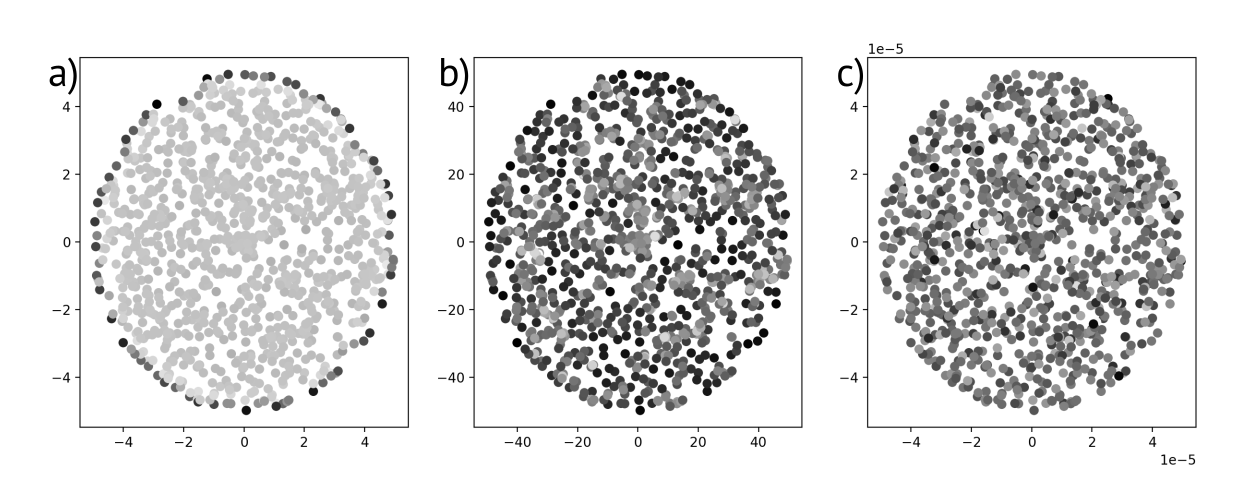
\includegraphics[width=\linewidth]{../figures/1_different_scales/plot_wlabels.png}
  \caption{Points sampled from a circle with radius $r=5$, scaled by $1$ (a), $10$ (b) and $10^{-5}$ (c). Points coloured according to weighting vector values taken from each circle separately, darker color indicates higher value.}
  \label{fig:diff_scales}
\end{figure}

\section{Experiments}

\subsection{Magnitude autoencoder}

While it is simple to observe the boundary of a two-dimensional dataset of points sampled from a circle, as shown in the example in the previous section, it takes more effort to visualize the boundary of a high-dimensional dataset. In order to plot the boundary in two-dimensional space, dimensionality reduction needs to be applied, which maps the high-dimensional input dataset to a two-dimensional representation. In addition, the boundary needs to be taken into account, which is represented by the  recently introduced weighting vector, which marks the boundaries of both the high-dimensional input and two-dimensional output datasets. The method chosen to perform dimensionality reduction is the autoencoder neural network, therefore we call the tool used to perform this specific task the Magnitude autoencoder.

The underlying basis of the investigations presented in this report is an autoencoder training strategy that focuses on the difference between the weighting vectors of the input and the dimensionally-reduced datasets. That is, in addition to minimizing the usual reconstruction loss term, in order to minimize the difference between the boundaries in the original and dimensionally-reduced datasets, we take the mean absolute difference between their weighting vectors into account. To be more precise, the autoencoder minimizes the sum of two loss terms. The first one is the reconstruction loss defined as the mean squared difference between the input dataset $X$ and the reconstructed, or output dataset $X'$: $$\mathcal{L}_{recons} = \frac{1}{n} ||X - X'||^{2}_{2}.$$ The second contribution to the total loss term is the mean absolute difference between the weighting vectors $w$ of the input dataset $X$ and its two-dimensional encoding $h$: $$\mathcal{L}_{weight} = \frac{1}{n} ||w_{X} - w_{h}||_{1}.$$ However, in our experiments we have observed that the use of mean squared difference in $\mathcal{L}_{weight}$ also produces similar results, so the definition of this loss term is not restricted to the mean absolute error proposed here. The total loss to be minimized is equal to $$\mathcal{L} = \mathcal{L}_{recons} + \lambda \mathcal{L}_{weight},$$ where $\lambda \in \mathbb{R}$ defines the impact of the weighting vector loss on the total loss.

\subsection{Network architecture}

The autoencoder was implemented using the $\itshape pytorch$ package (\cite{NEURIPS2019_9015}). The neural network is composed of two parts: encoder and decoder. The encoder takes the $n$-dimensional vector as input and outputs a two-dimensional vector, which is the dimensionally-reduced output we are interested in from a trained network. The decoder does the opposite by aiming to reconstruct the input vector using its two-dimensional representation. Two neural network architectures are used in the experiments presented in this report.

The first one will be referred to as the Linear autoencoder. Its first half, the encoder, consists of seven linear layers: the first six have 64 outputs, the seventh layer has 64 inputs and 2 outputs, returning the dimensionally reduced representation. The encoder has the same but reverse (2-64-64-64-64-64-64-n) architecture. Instead of  Rectified (ReLU),  Sigmoid Linear Units (SiLU) (\cite{Hendrycks2016}) are used as activation functions due to the nature of the weighting vector loss term $\mathcal{L}_{weight}$. During our experiments, we noticed that while training the neural network, multiple activation values can become exactly equal to $0$, which might lead to a scenario where multiple different points in the input dataset are mapped to the same point in the two-dimensional space. This causes the similarity matrix of the two-dimensional dataset to become singular, and the calculation of its inverse fails. Using SiLU solves this problem, since it is not constantly $0$ for negative input values, and this results in different points from the initial high-dimensional space being mapped to different points in the two-dimensional space.

The second autoencoder will be referred to as the Convolutional autoencoder, which was used to perform dimensionality reduction for an image dataset. The architecture used to generate the results in this report was mostly based on a previous implementation of a convolutional autoencoder (\cite{Moor2019}), originally defined as class $\itshape ConvolutionalAutoencoder\_2D$. The implementation is modified slightly by changing the architecture of the linear layers of the autoencoder to (576-1000-500-250-2-250-500-1000) and by replacing the ReLU activation functions by SiLU, while the convolutional layers of the architecture were left unchanged. In the encoder, the first two layers are $\itshape Conv2d$ layers with 1 and 8 input channels, 8 and 4 output channels, respectively, and the kernel size of 9 in both layers. In the decoder, the last layer is a $\itshape Conv2d$ layer with 4 input channels, a single output channel and a kernel of size 1. The two layers preceding the last one are $\itshape ConvTranspose2d$ layers with 1000 and 4 input channels, 4 output channels, and kernels of sizes 12 and 17, respectively. Additionally, the output of the decoder is passed through a $\itshape Tanh$ activation function.

In all experiments presented in this report, the autoencoder was trained using the ADAM (\cite{Kingma2014}) optimizer with the weight decay parameter set to $10^{-5}$. The learning rate parameter was set to $10^{-2}$ for the Linear autoencoder and $10^{-3}$ for the Convolutional autoencoder.

\subsection{Training inefficiencies}

While we have defined the optimization goal, minimization of such a loss function causes problems in the autoencoder training. The main issue is that the boundary of a dataset is a global property. This means that the weighting vector of a subset of the dataset does not outline the boundary of the whole. Therefore, the calculation of the weighting vector has to take all the points in the dataset into account at once.

The inability to decompose autoencoder training epochs into multiple smaller batches is a serious limitation, since, while it is necessary to use the whole dataset for the weighting vector loss minimization, it also makes reconstruction loss minimization very inefficient, since it would significantly benefit from multiple smaller batches per epoch. The general approach to this would be to perform the reconstruction loss minimization separately from the weighing vector loss.

One way to achieve this could be the "predictor-corrector" strategy. It involves training the network to efficiently minimize the reconstruction loss using small batches, then "correcting" the network by training it only to minimize the weighting vector loss. These two steps would be repeated one after the other until convergence. Unfortunately, such a procedure can be very unstable, as the progress done by one step is likely to be offset by the next step. This was the case in our experiments, as each training step would simultaneously lower the value of one loss term and raise the value of the other one, thus resulting in no total loss $\mathcal{L}$ minimization overall. We had more success with a different strategy, which incorporates a "burn-in" procedure. Initially, the autoencoder is trained to minimize only the reconstruction loss using small batches. When this is done, the total loss $\mathcal{L}$ is minimized as before, using a single batch per epoch. The subsequent minimization of total loss $\mathcal{L}$ will most likely raise the value of reconstruction loss, since the weighting vector loss is minimized also. However, the starting point for $\mathcal{L}$ minimization is improved, since the reconstruction loss minimization is already partially done.
% weird sentence ^

On the other hand, the calculation of the weighting vector is very time consuming for large datasets. For a dataset composed of $n$ elements, it involves the inversion of a $n$ by $n$ matrix, time complexity of this operation is $O(n^3)$. Three methods were investigated to make the weighting vector calculation more efficient. The first method involves the Schur complement (\cite{Bunch2021}), which allows to split the input matrix into a block matrix, effectively allowing to split the input dataset into two parts, for which the weighting vector is calculated separately. Unfortunately, this procedure can not be applied recursively, only a single split can be done. Additionally, our implementation of the algorithm was as efficient as the matrix inversion function implemented in the $\itshape{pytorch}$ package. The second method we looked into makes use of the fact that the matrix we need to invert is a similarity matrix (\cite{Ambikasaran2014}), which claims time complexity of $O(n \log{n})$. However, this method is originally implemented in C++. Any calculations done in the context of $\itshape pytorch$ need to be implemented using objects and operations native to $\itshape pytorch$. Therefore, in order to make use of this algorithm in our case, it would have to be rewritten using $\itshape pytorch$ C++ API. The third method to speed up the calculation of the weighting vector is the one we employed, which involves solving a linear system of equations instead of performing the matrix inversion: $$\text{Solve } \zeta_{X} w_{X} = \mathds{1} \text{ like } Ax = b.$$ While the time complexity of this operation is also $O(n^{3})$, in our experiments we have observed that calculating the weighting vector $w_{X}$ directly in this way is about $4$ times faster that using matrix inversion.

\subsection{Basic shapes}

In order to see how the previously defined autoencoder works in principle, we apply the Linear autoencoder to three datasets representing shapes with qualitatively different boundaries.

\begin{itemize}
    \item Swiss roll
    \item Sphere
    \item Ball
\end{itemize}

To make the problem easy to visualize, the high-dimensional input data is composed of points in three-dimensional space. Each of the three datasets consists of $1000$ points which are uniformly sampled from the corresponding shapes. The datasets representing the Swiss roll and the sphere shapes were generated using the $\itshape tadasets$ package (\cite{scikittda2019}).The results can be see in Figure \ref{fig:basic_shapes}. The performance of the autoencoder can be assessed visually by using the weighting vector of the three-dimensional input dataset to color the points in the dimensionally-reduced dataset. A desired result is one where the autoencoder maps the boundary points from the three-dimensional dataset, which have a high weighting score and are of a darker color, to the boundary of the dimensionally-reduced dataset.

The first shape to look into is the Swiss roll, generated with parameters $r=3$ and $\text{noise}=0.03$. It is a two-dimensional surface, therefore, its boundary can be easily mapped to a two-dimensional plane, therefore, it is used to check if the autoencoder manages to function in the most basic scenario. As we see in the first column of Figure \ref{fig:basic_shapes}, the boundary-preserving dimensionality reduction is successful, since the  points on the boundary of the two-dimensional representation, based on their color, are also boundary points in the original dataset. 

The next object is the sphere with radius $r=20$ (second column in Figure \ref{fig:basic_shapes}). The shape is composed purely out of boundary points, and the autoencoder is again able to preserve the weighting vector from the input dataset in the dimensionally-reduced dataset. Additionally, even though the points are sampled uniformly from a sphere, two small clusters of points are present on opposite poles of the sphere. These two structures are also present in the dimensionally-reduced representation, which suggests that boundary preservation using $\mathcal{L}_{weight}$ minimization might also play a role in the preservation of the underlying structures in the original data.

The last and conceptually most difficult shape to deal with is the ball, generated by uniformly sampling points from a ball with radius $r=2$ (third column in Figure \ref{fig:basic_shapes}), and the autoencoder is unable to move all of the boundary points in the input dataset to the boundary of the dimensionally-reduced dataset. This can be seen by observing that the two-dimensional representation contains points in its interior, which have high weighting scores in the input dataset. This is not unexpected, since matching the boundaries between the two representations would require mapping the boundary points, which represent a sphere, to a circle, which would lead to a significant loss of structure-related information in the two-dimensional representation. 

However, visual inspection is not enough to determine how well the Magnitude autoencoder functions. In order to quantify the success of the boundary preservation we compute the Pearson correlation coefficient between the weighting vector of the points in the input space and two-dimensional space. For the Swiss roll, sphere and ball the correlations are 0.96, 0.94 and 0.52, respectively. Additionally, results of other dimensionality reduction methods, PCA and t-SNE (\cite{t-SNE}), are given in rows 3 and 4 of Figure \ref{fig:basic_shapes}. Using the Pearson correlation coefficient criterion, in all three examples the Magnitude autoencoder performs best. However, the two-dimensional representation returned by the Magnitude autoencoder received only a slightly higher score than the result obtained using PCA.

\begin{figure}
  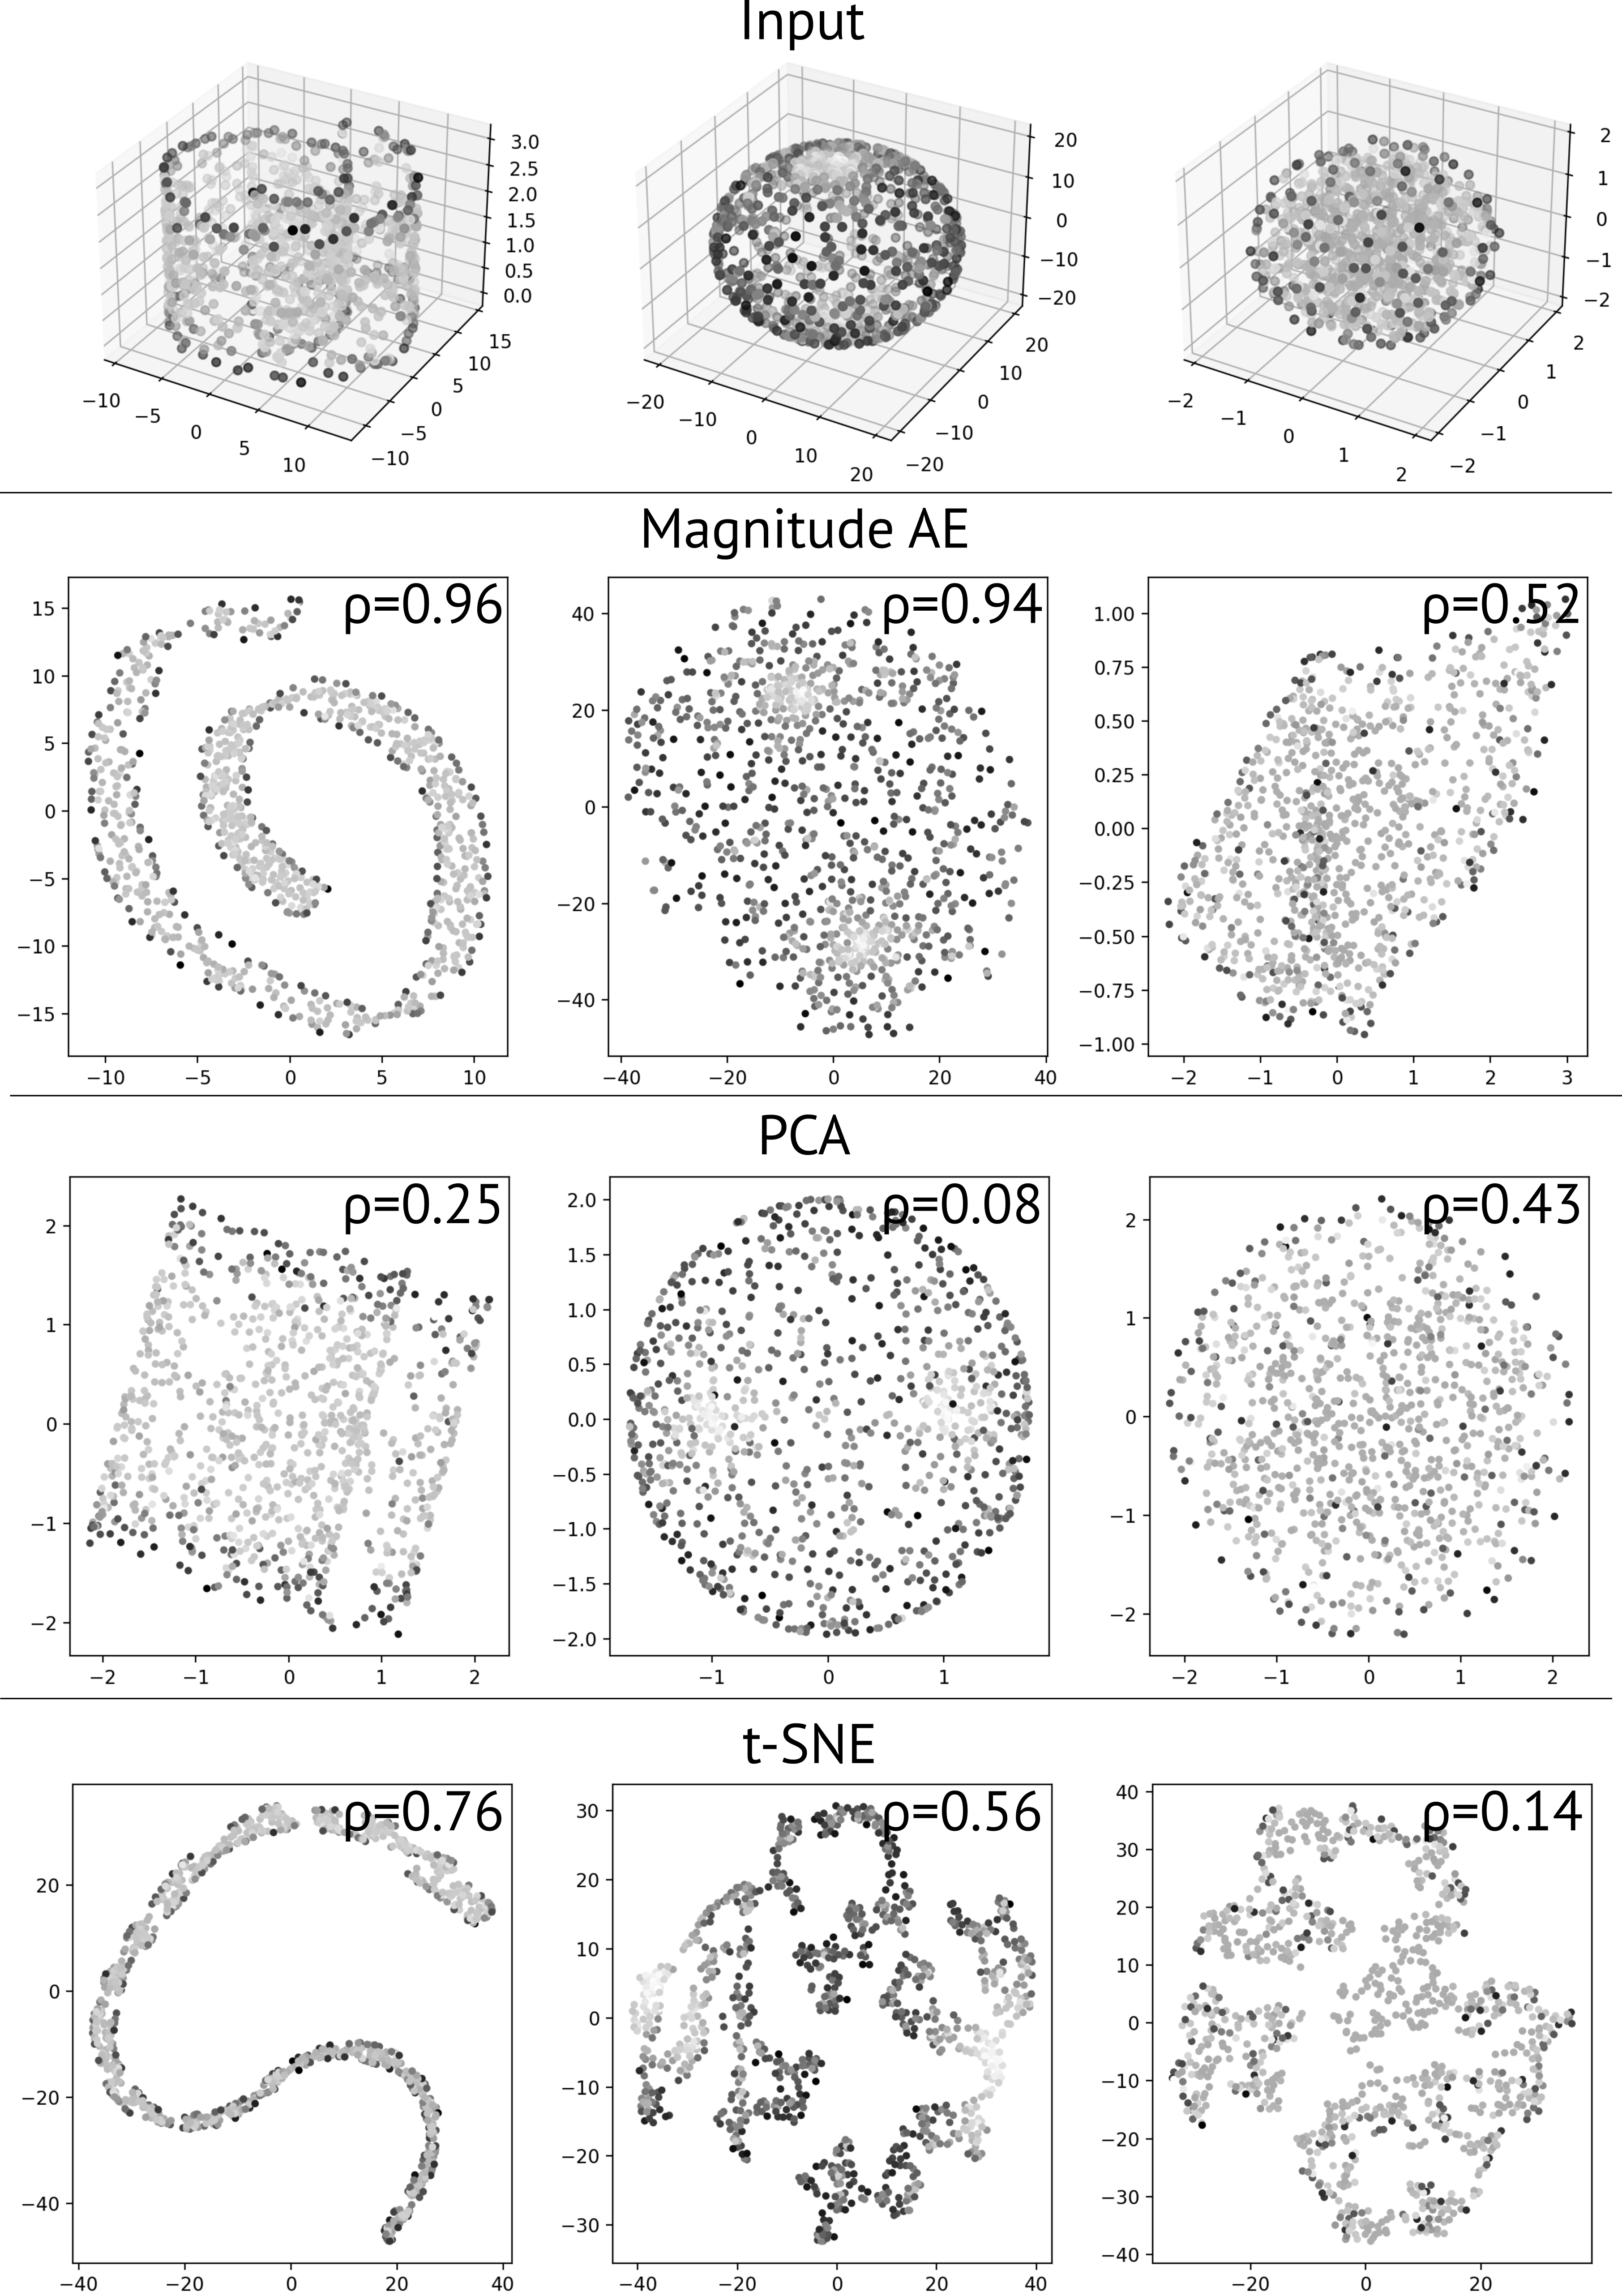
\includegraphics[width=\linewidth]{../figures/2_basic_shapes/plot_wlabels.png}
  \caption{Dimensionality reduction results for the three shapes: Swiss roll (first column), sphere (second column) and ball (third column). The plots in the first row show the input datasets with points colored according to the weighting vector values of these datasets. The plots in the other rows show the two-dimensional representations of the corresponding datasets with points colored according to the weighting vector values of the input datasets. The $\rho$ values indicate the Pearson correlation coefficients between the weighting vectors of the input and dimensionally-reduced datasets.}
  \label{fig:basic_shapes}
\end{figure}

\subsection{Additional model parameters}

In order to achieve the results shown in the previous section, two training parameters had to be adjusted, which are supplied in addition to the input data.

The first one is the multiplier $\lambda$, which specifies how large the impact of the weighting vector loss is on the total loss $\mathcal{L}_{recons} + \lambda \mathcal{L}_{weight}$. Initially, our guess was that increasing the value of this parameter would increase the reconstruction loss $\mathcal{L}_{recons}$ and decrease the weighting vector loss $\mathcal{L}_{weight}$, and this would complicate the choice of $\lambda$. However, when we investigate how the values of these losses depend on different $\lambda$ values for the Swiss roll dataset, we see that $\mathcal{L}_{recons}$ is not minimized when $\lambda$ is set to zero (Figure \ref{fig:additional_parameters}.a). Additionally, at least for this dataset, for a pair of values ($\lambda \in \{5, 10\}$), both loss terms are minimized, therefore, we do not need to make a choice on which loss term of the two we would like to minimize. However, the optimization of $\lambda$ for every dataset might not be crucial, since the same value of 5 was used in all examples shown in this report with some success.

The other parameter is directly related to the input dataset, since it defines its scale. As mentioned before, if we have a dataset $X$, we can use a rescaling factor $t$ to get a new dataset $tX$, which has the same points as $X$, but the distances between them are $t$ times larger. Then, if $t$ is large enough, the magnitude of $X$ becomes close to the number of points $|X|$, and the weighting score of each point in $X$ gains a value close to 1. Therefore, for a given dataset, we need to find a proper rescaling factor $t$, with which the dataset $tX$ has a clearly defined boundary, with higher weighting scores assigned to points on the boundary. If we take the same Swiss roll dataset as an example, it is easy to visualize the results of using different rescaling factors to see which one results in a desirable weighting vector. However, for truly high-dimensional datasets we might not be sure whether the weighting vector highlights the boundary of the dataset. Fortunately, the choice of the rescaling factor might not be arbitrary, as can be seen in Figure \ref{fig:additional_parameters}.b. For higher values of the rescaling factor, where a boundary no longer exists and the distribution of weighting scores over points is uniform, the training loss value $\mathcal{L}$ also becomes increasingly larger. Also, the value of $t$ minimizing the loss $\mathcal{L}$ is one with which the boundary of the dataset is clearly highlighted by the weighting vector. This observation is useful, since it suggests that the autoencoder training performance can be used to determine whether the scale of the input dataset is appropriate, that is, whether the weighting vector is able to highlight its boundary points.

\begin{figure}
  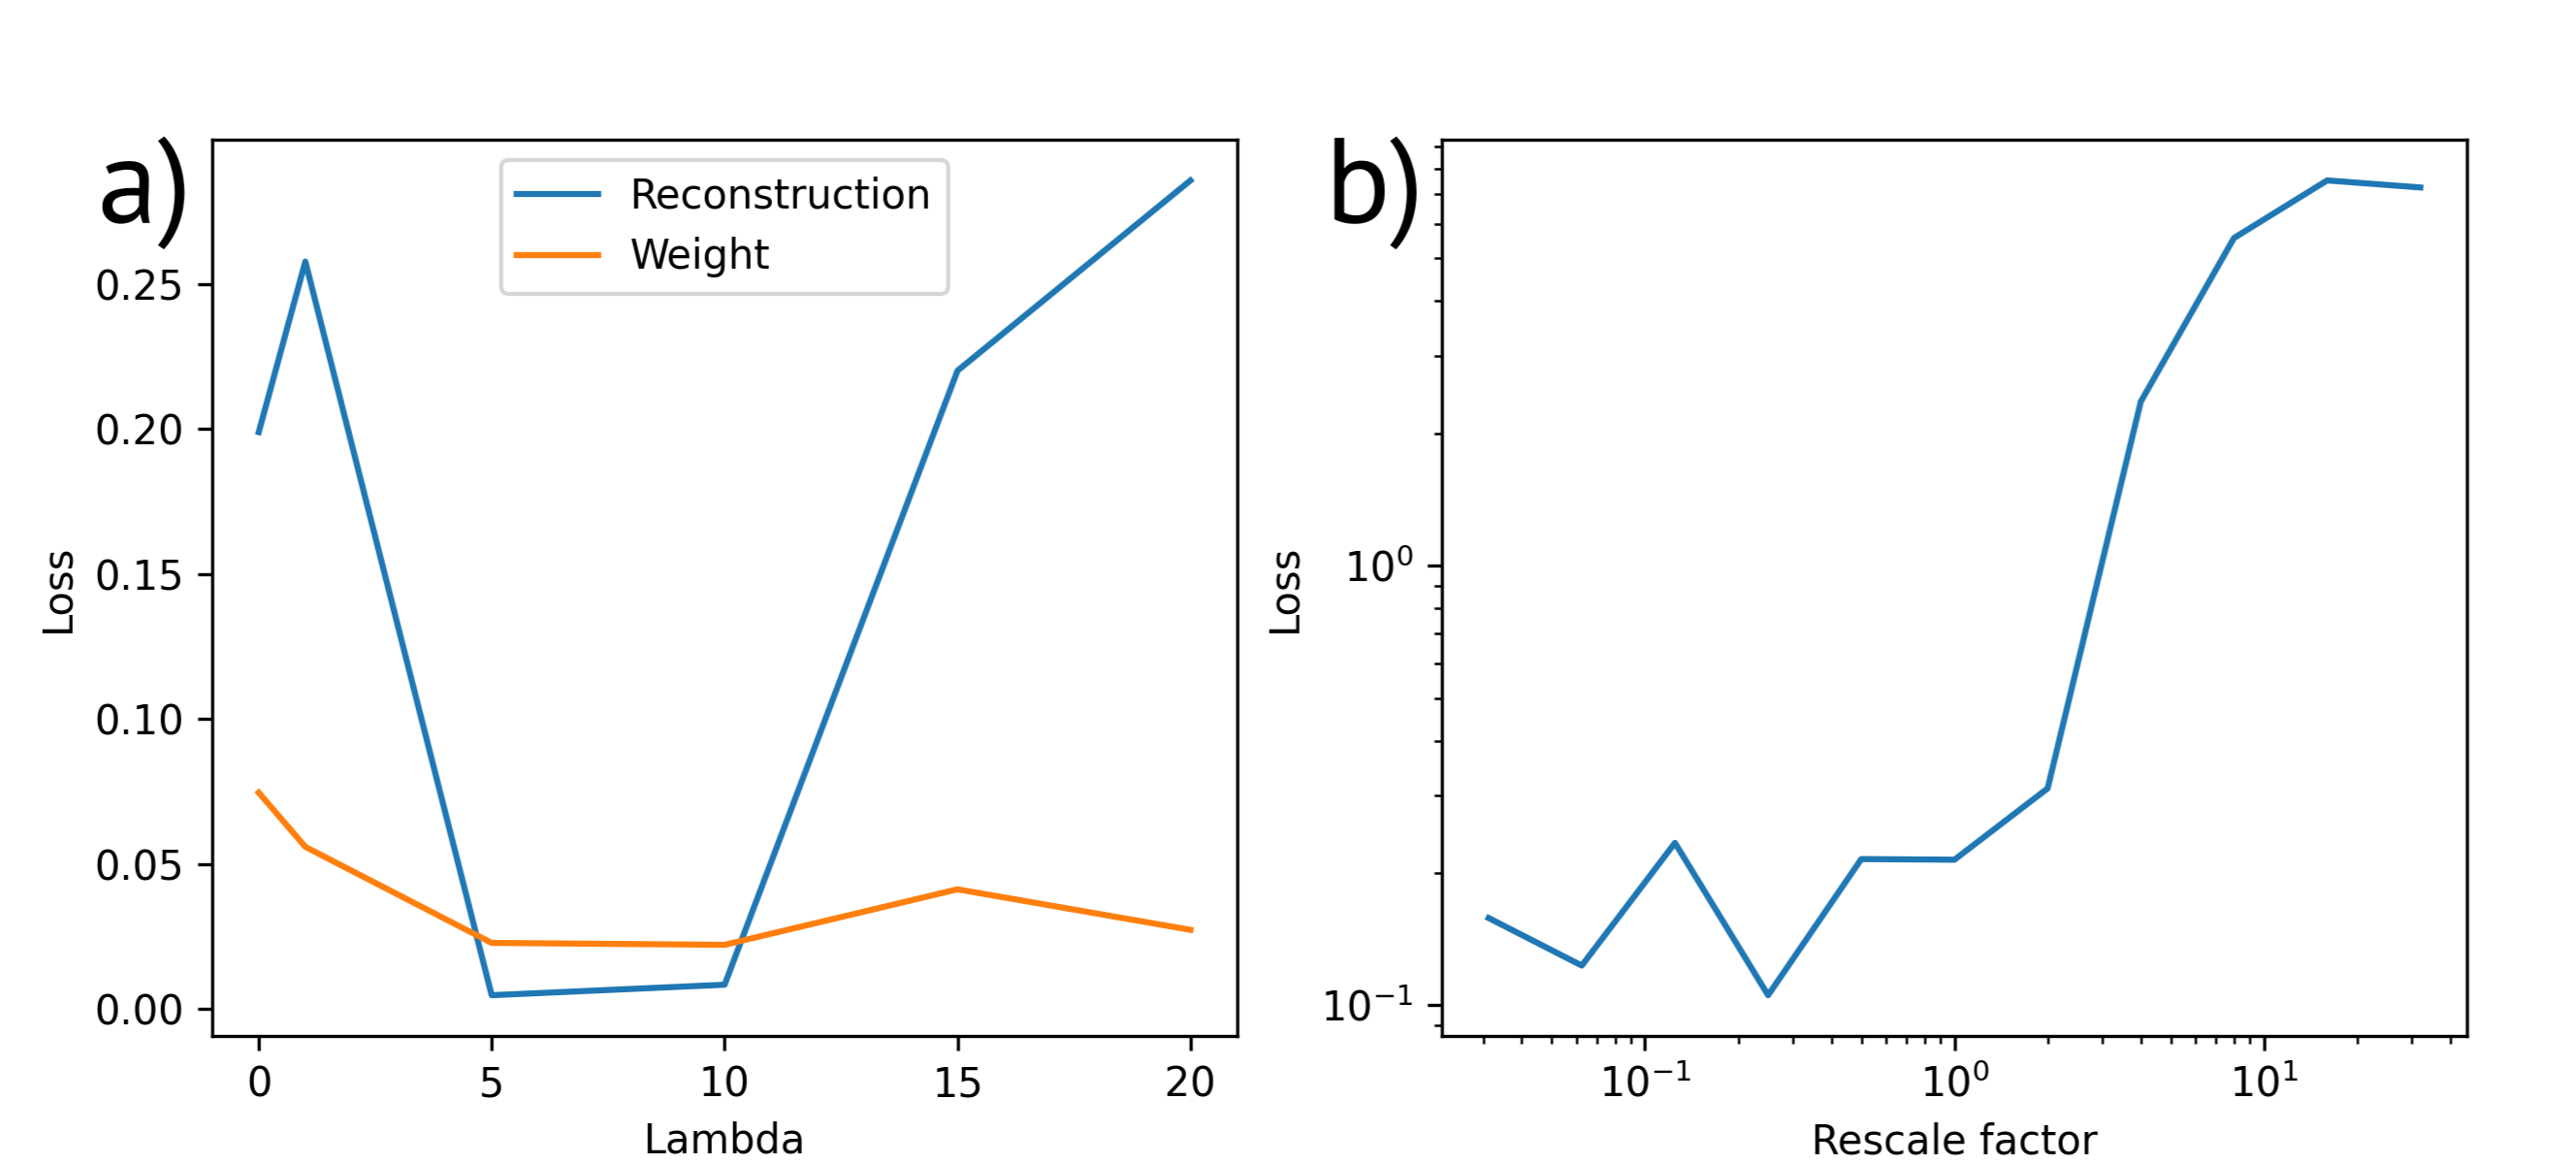
\includegraphics[width=\linewidth]{../figures/3_additional_parameters/plot_wlabels.png}
  \caption{Loss values obtained from training the autoencoder on the Swiss roll dataset with different parameter $\lambda$
  (a) and $t$ (b) values.}
  \label{fig:additional_parameters}
\end{figure}

\subsection{MNIST dataset}

After seeing that the proposed autoencoder training strategy in principle works on simple datasets, we can look into a real-world example - the MNIST dataset of handwritten digits (\cite{Lecun1998}), obtained using the $\itshape torchvision$ package. The full dataset is composed of 60,000 points, and in order to speed up the computations, 3000 points, or one twentieth of the dataset is used. Since the input points are images, instead of the previously used Linear autoencoder architecture, the other previously described Convolutional autoencoder architecture is employed. Additionally, due to the large size of the dataset, the minimization of $\mathcal{L}_{recons}$ becomes very inefficient, so the previously defined "burn-in" strategy is employed. First, the autoencoder is trained for a few epochs with multiple small batches per epoch minimizing only the reconstruction loss. After this "burn-in" procedure is done, the previous strategy of minimizing the sum of the two loss terms is employed.

Since the dataset is truly high-dimensional, unlike the previous examples, we are unable to observe whether the weighting vector highlights the boundary points properly, therefore a proper rescaling factor needs to be chosen. Various rescaling factors in the interval $(0, 1)$ were applied, and no apparent relationship like the one shown in Figure \ref{fig:additional_parameters}.b between the rescaling factor values and $\mathcal{L}$ was observed. However, for all but one rescaling factor value (equal to $0.6$) the reduction in $\mathcal{L}$ was minimal relative to the loss value at the start of training, after the "burn-in" procedure. The training results with $t=0.6$ after the "burn-in" procedure are shown in Figure \ref{fig:mnist}.a, where the initial weighting vector loss is reduced by around 40\% after 46 training epochs.

To evaluate the success of dimensionality reduction, we can again use the Pearson correlation coefficient between the weighting vectors of the input and dimensionally-reduced data. In this case, it is equal to 0.72 (Figure \ref{fig:mnist}.b), which, compared to the previous examples, could be considered an acceptable result, taking into account the more arbitrary structure of the dataset and significantly higher dimensionality. Results obtained using two other dimensionality reduction techniques, PCA and t-SNE, are also added for comparison. While t-SNE is able to separate different categories in the dataset, PCA is more successful at boundary preservation with a correlation value of 0.49. The Magnitude autoencoder is able to both retain the boundary in the two-dimensional space, and it is also more successful than PCA in clustering the separate categories, as can be seen in overlapping clouds of points belonging to the same category.

\begin{figure}
  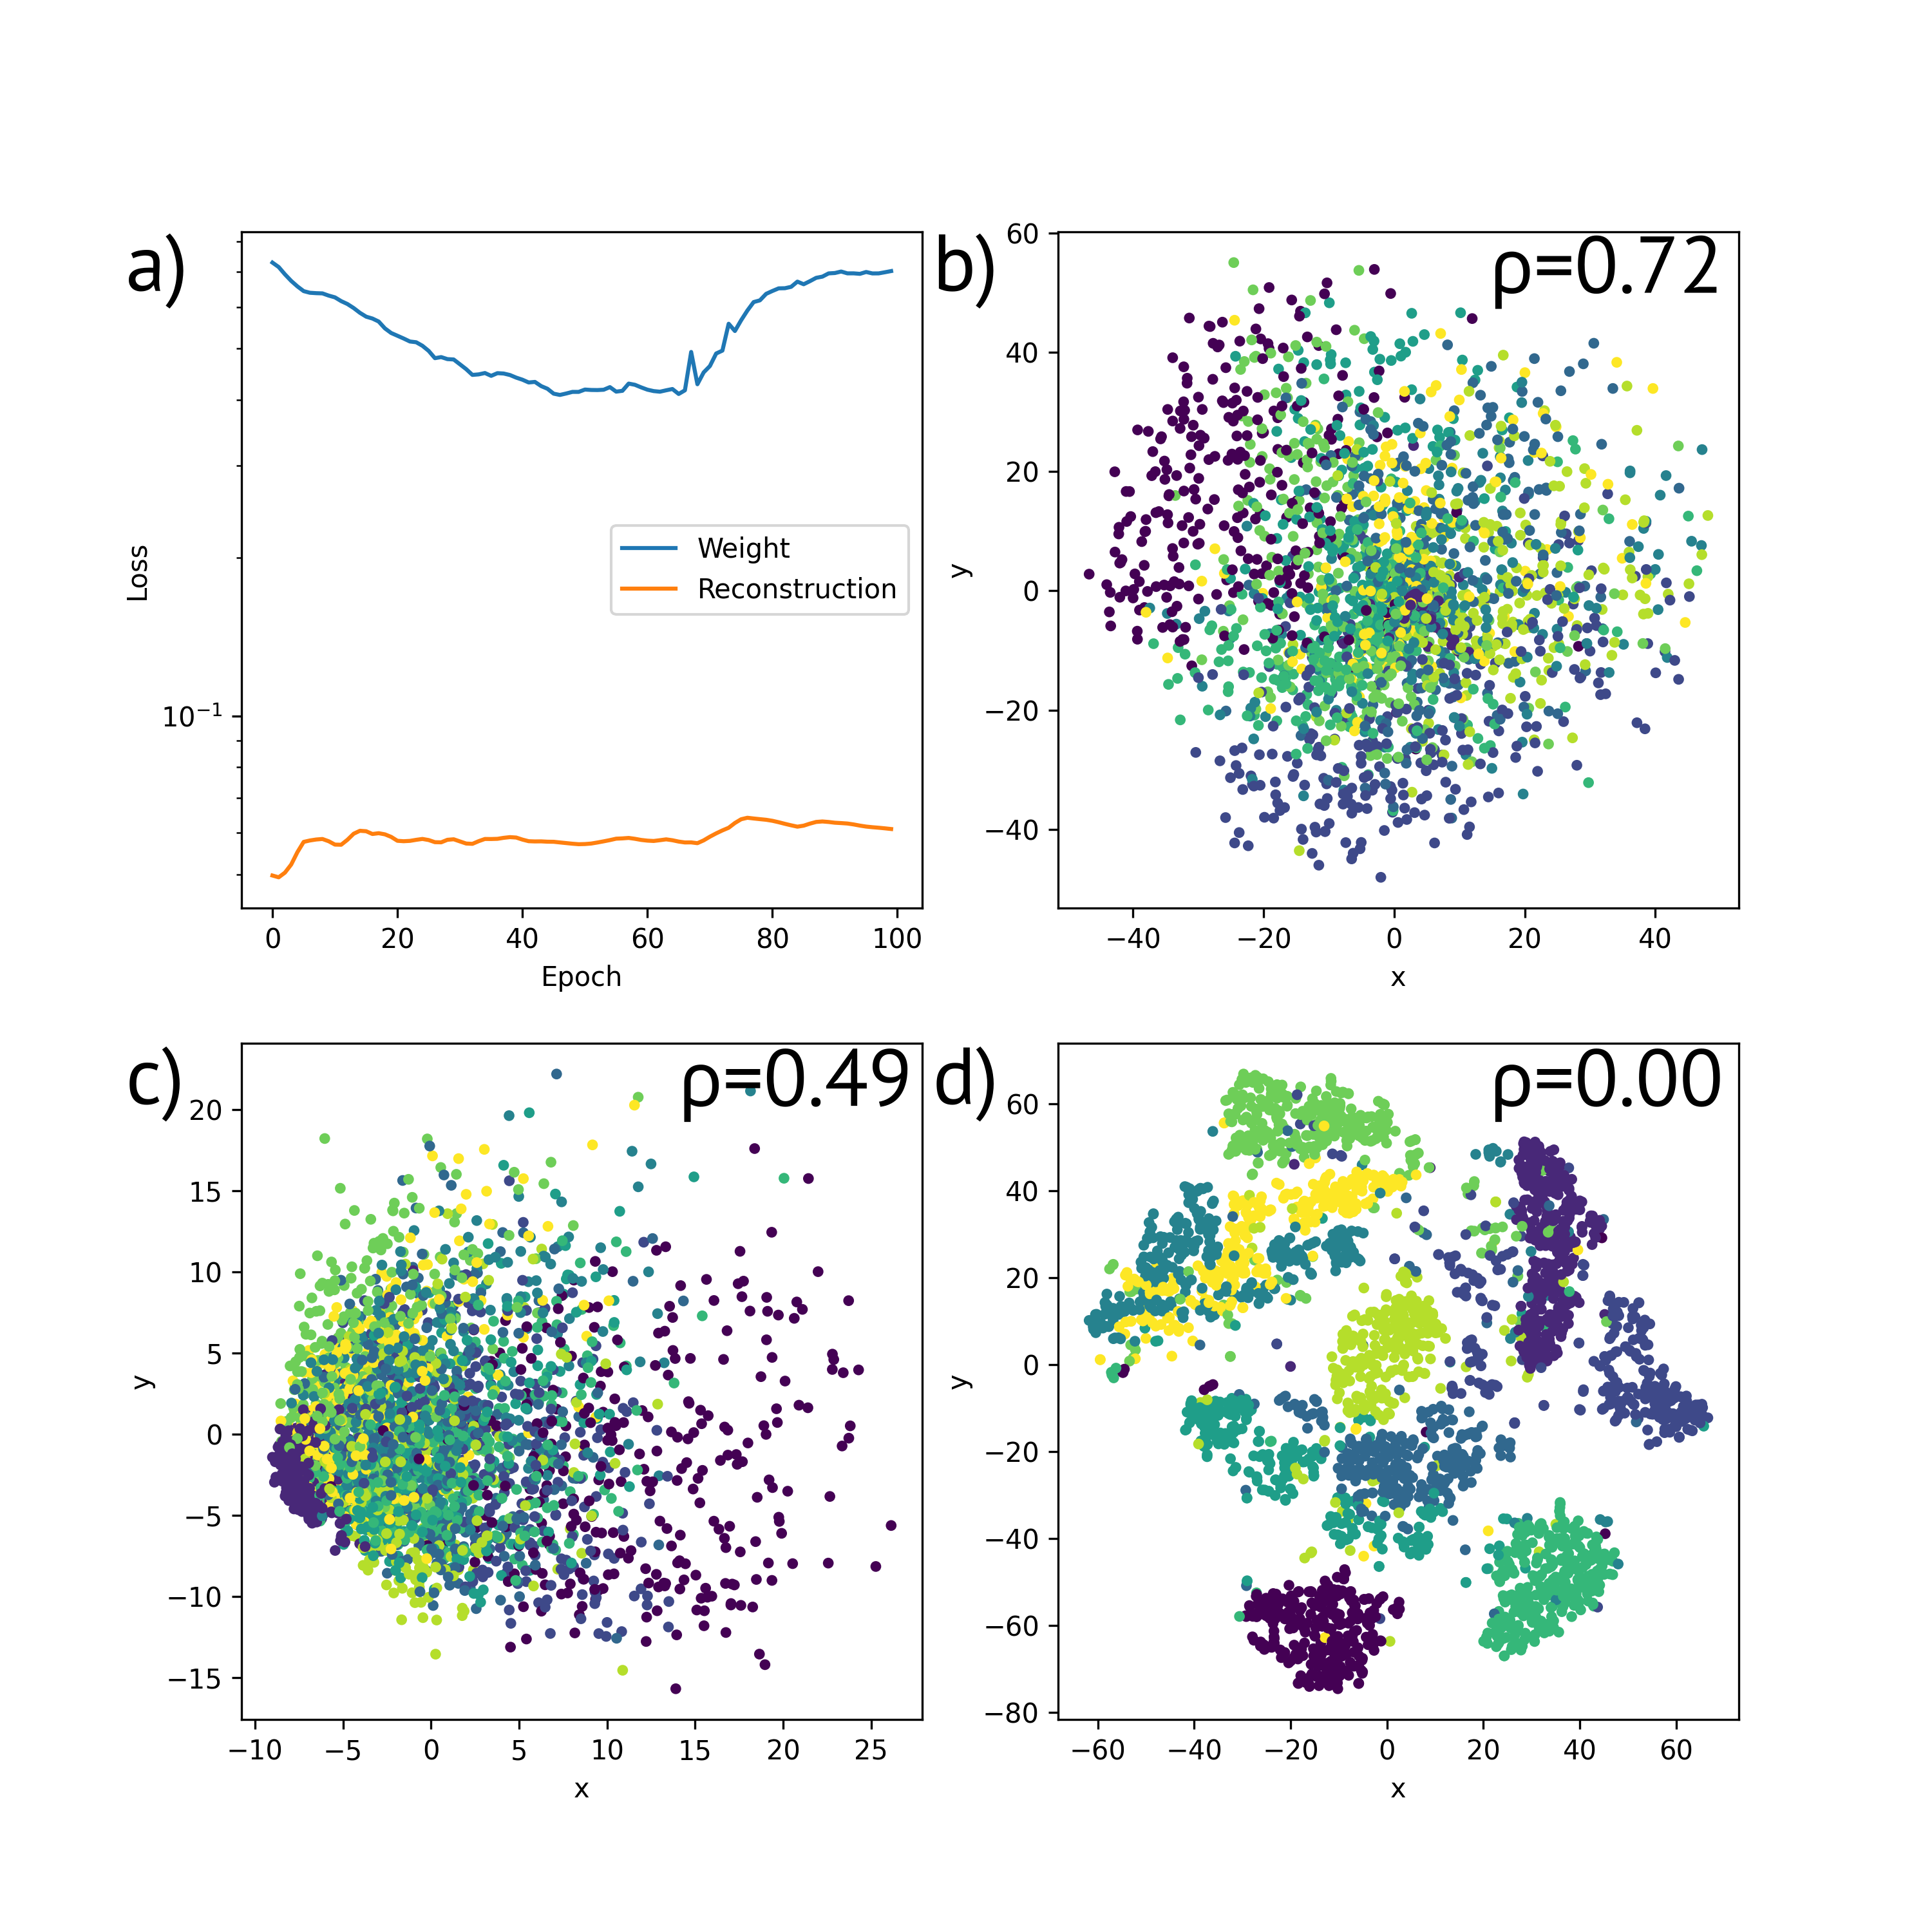
\includegraphics[width=\linewidth]{../figures/4_mnist/plot_wlabels.png}
  \caption{Results obtained from training the autoencoder on the MNIST dataset. The first plot shows how the values of $\mathcal{L}_{recons}$and $\mathcal{L}_{weight}$ loss terms change over training epochs (a). The next three plots show dimensionality reduction results with points colored according to their class: after 46 training epochs using the Magnitude autoencoder (b), PCA (c), t-SNE (d). The $\rho$ values indicate the Pearson correlation coefficients between the weighting vectors of the input and dimensionally-reduced datasets.}
  \label{fig:mnist}
\end{figure}

\section{Conclusion}

The examples shown in the report demonstrate that a boundary of a high-dimensional dataset can be mapped to a two-dimensional space. This can be done using an autoencoder neural network with a simple loss function, which takes the boundary of a dataset into account by focusing on its weighting vector. The examples included highly-structured datasets representing basic geometric shapes, and a more arbitrary dataset of handwritten digit images, and the initially proposed training strategy showed at least some success in all examples.

However, the autoencoder training method presented here is overly simplistic - for large datasets it effectively involves multiple inversions of large similarity matrices. This can be prohibitively time consuming, and the large number of points might also reduce the efficiency of single training epochs.

Fortunately, the efficiency of the autoencoder training can be significantly improved by using a better matrix inversion algorithm, like the one specifically tailored for similarity matrices (\cite{Ambikasaran2014}). However, to assess the actual performance of the algorithm for our use case, it first needs to be reimplemented in the $\itshape pytorch$ environment.

Additionally, there still might be a way to simplify the minimization of the weighting vector loss $\mathcal{L}_{weight}$ by using smaller subsets of the dataset. After seeing how important scale of the input dataset is to the minimization of the overall loss $\mathcal{L}$, it would be useful to investigate whether rescaling of the small batches can improve or even enable $\mathcal{L}_{weight}$ minimization using multiple small batches instead of the whole dataset.

The source code used to produce the report and the results presented in it can be found at \href{https://github.com/tadasbar/Magnitude-autoencoder}{https://github.com/tadasbar/Magnitude-autoencoder}.

\printbibliography

\end{document}
